\documentclass{article}

% packages
\usepackage{amsmath, amsthm, thmtools, amsfonts, amssymb, luacode, catchfile, tikzducks, hyperref, ifthen}
\ifcsname c@kobocompile\endcsname
	\usepackage[a5paper, total={1072pt, 1448pt}, margin=10pt, includeheadfoot]{geometry} % set page margins
\else
	\usepackage[a4paper, margin=50pt, includeheadfoot]{geometry}
\fi
\usepackage[shortlabels]{enumitem}
\usepackage[skip=3pt, indent=0pt]{parskip}

% language
\usepackage[bidi=basic, layout=tabular, provide=*]{babel}
\ifcsname c@english\endcsname
	\babelprovide[main, import]{english}
\else
	\babelprovide[main, import]{hebrew}
	\babelprovide{rl}
\fi
%\babelfont{rm}{Libertinus Serif}
\babelfont{rm}[Renderer=Harfbuzz]{Libertinus Serif}
\babelfont{sf}{Libertinus Sans}
\babelfont{tt}{Libertinus Mono}

% style
\AddToHook{cmd/section/before}{\clearpage}	% Add line break before section
\linespread{1.3}
\setcounter{secnumdepth}{0}		% Remove default number tags from sections, this won't do well with theorems
\AtBeginDocument{\setlength{\belowdisplayskip}{3pt}}
\AtBeginDocument{\setlength{\abovedisplayskip}{3pt}}
\graphicspath{ {../images/} }

% operators
\DeclareMathOperator\cis{cis}
\DeclareMathOperator\Sp{Sp}
\DeclareMathOperator\tr{tr}
\DeclareMathOperator\im{Im}
\DeclareMathOperator\re{Re}
\DeclareMathOperator\diag{diag}
\DeclareMathOperator*\lowlim{\underline{lim}}
\DeclareMathOperator*\uplim{\overline{lim}}
\DeclareMathOperator\rng{rng}
\DeclareMathOperator\Sym{Sym}
\DeclareMathOperator\Arg{Arg}
\DeclareMathOperator\Log{Log}
\DeclareMathOperator\dom{dom}
\DeclareMathOperator\supp{Supp}
\DeclareMathOperator\var{Var}
\DeclareMathOperator\cov{Cov}

% commands
%\renewcommand\qedsymbol{\textbf{מש''ל}}
%\renewcommand\qedsymbol{\fbox{\emoji{lizard}}}
\newcommand{\Aa}[0]{\mathcal{A}}
\newcommand{\Bb}[0]{\mathcal{B}}
\newcommand{\CC}[0]{\mathbb{C}}
\newcommand{\Cc}[0]{\mathcal{C}}
\newcommand{\EE}[0]{\mathbb{E}}
\newcommand{\FF}[0]{\mathbb{F}}
\newcommand{\Ff}[0]{\mathcal{F}}
\newcommand{\Ii}[0]{\mathcal{I}}
\newcommand{\Gg}[0]{\mathcal{G}}
\newcommand{\Ll}[0]{\mathcal{L}}
\newcommand{\Mm}[0]{\mathcal{M}}
\newcommand{\NN}[0]{\mathbb{N}}
\newcommand{\Nn}[0]{\mathcal{N}}
\newcommand{\PP}[0]{\mathbb{P}}
\newcommand{\Pp}[0]{\mathcal{P}}
\newcommand{\QQ}[0]{\mathbb{Q}}
\newcommand{\RR}[0]{\mathbb{R}}
\newcommand{\Rr}[0]{\mathcal{R}}
\newcommand{\Ss}[0]{\mathcal{S}}
\newcommand{\TT}[0]{\mathbb{T}}
\newcommand{\Uu}[0]{\mathcal{U}}
\newcommand{\Vv}[0]{\mathcal{V}}
\newcommand{\Ww}[0]{\mathcal{W}}
\newcommand{\ZZ}[0]{\mathbb{Z}}
\newcommand{\acts}[0]{\circlearrowright}
\newcommand{\explain}[2] {
	\begin{flalign*}
		 && \text{#2} && \text{#1}
	\end{flalign*}
}
\newcommand{\maketitleprint}[0]{ \begin{center}
	%\begin{tikzpicture}[scale=3]
	%	\duck[graduate=gray!20!black, tassel=red!70!black]
	%\end{tikzpicture}	
	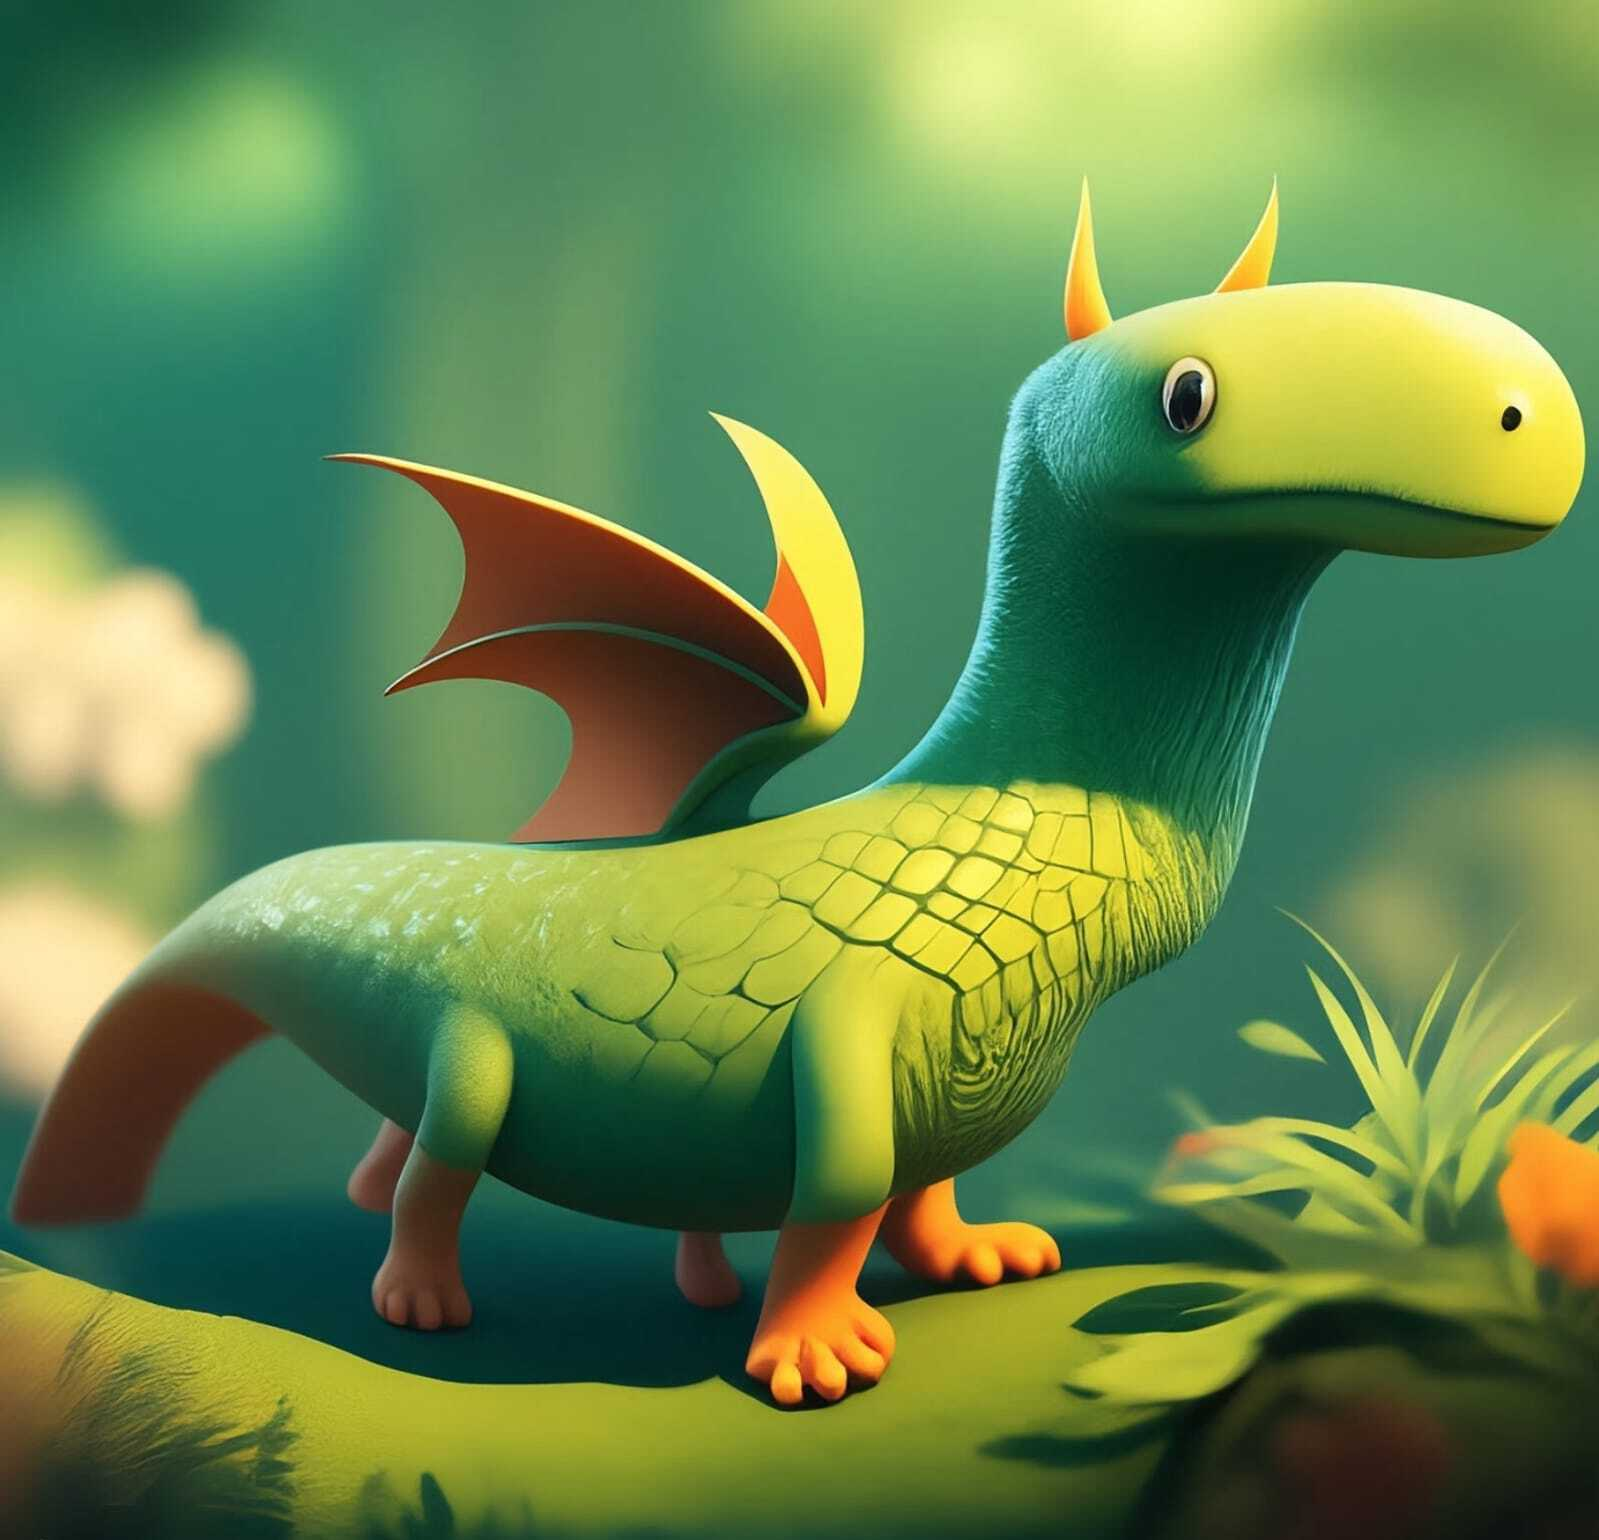
\includegraphics[width=6cm]{cover}
\end{center}
}

% theorem commands
\newtheoremstyle{c_remark}
	{}	% Space above
	{}	% Space below
	{}% Body font
	{}	% Indent amount
	{\bfseries}	% Theorem head font
	{}	% Punctuation after theorem head
	{.5em}	% Space after theorem head
	{\thmname{#1}\thmnumber{ #2}\thmnote{ \normalfont{\text{(#3)}}}}	% head content
\newtheoremstyle{c_definition}
	{3pt}	% Space above
	{3pt}	% Space below
	{}% Body font
	{}	% Indent amount
	{\bfseries}	% Theorem head font
	{}	% Punctuation after theorem head
	{.5em}	% Space after theorem head
	{\thmname{#1}\thmnumber{ #2}\thmnote{ \normalfont{\text{(#3)}}}}	% head content
\newtheoremstyle{c_plain}
	{3pt}	% Space above
	{3pt}	% Space below
	{\itshape}% Body font
	{}	% Indent amount
	{\bfseries}	% Theorem head font
	{}	% Punctuation after theorem head
	{.5em}	% Space after theorem head
	{\thmname{#1}\thmnumber{ #2}\thmnote{ \text{(#3)}}}	% head content

\ifcsname c@english\endcsname
	\theoremstyle{plain}
	\newtheorem{theorem}{Theorem}[section]
	\newtheorem{lemma}[theorem]{Lemma}
	\newtheorem{proposition}[theorem]{Proposition}
	\newtheorem*{proposition*}{Proposition}
	%\newtheorem{corollary}[theorem]{אין חלופה עברית}

	\theoremstyle{definition}
	\newtheorem{definition}[theorem]{Definition}
	\newtheorem*{definition*}{Definition}
	\newtheorem{example}{Example}[section]
	\newtheorem{exercise}{Exercise}[section]

	\theoremstyle{remark}
	\newtheorem*{remark}{Remark}
	\newtheorem*{solution}{Solution}
	\newtheorem{conclusion}[theorem]{Conclusion}
	\newtheorem{notation}[theorem]{Notation}
\else
	\theoremstyle{c_plain}
	\newtheorem{theorem}{משפט}[section]
	\newtheorem{lemma}[theorem]{למה}
	\newtheorem{proposition}[theorem]{טענה}
	\newtheorem*{proposition*}{טענה}
	%\newtheorem{corollary}[theorem]{אין חלופה עברית}

	\theoremstyle{c_definition}
	\newtheorem{definition}[theorem]{הגדרה}
	\newtheorem*{definition*}{הגדרה}
	\newtheorem{example}{דוגמה}[section]
	\newtheorem{exercise}{תרגיל}[section]

	\theoremstyle{c_remark}
	\newtheorem*{remark}{הערה}
	\newtheorem*{solution}{פתרון}
	\newtheorem{conclusion}[theorem]{מסקנה}
	\newtheorem{notation}[theorem]{סימון}
\fi

% Questions related commands
\newcounter{question}
\setcounter{question}{1}
\newcounter{sub_question}
\setcounter{sub_question}{1}

\ifcsname c@english\endcsname
	\newcommand{\question}[1][0]{
		\ifthenelse{#1 = 0}{}{\setcounter{question}{#1}}
		\section{Question \arabic{question}}
		\addtocounter{question}{1}
		\setcounter{sub_question}{1}
	}

	\newcommand{\subquestion}[1][0]{
		\ifthenelse{#1 = 0}{}{\setcounter{sub_question}{#1}}
		\subsection{Part \alph{sub_question}}
		\addtocounter{sub_question}{1}
	}
\else
	\newcommand{\question}[1][0]{
		\ifthenelse{#1 = 0}{}{\setcounter{question}{#1}}
		\section{שאלה \arabic{question}}
		\addtocounter{question}{1}
		\setcounter{sub_question}{1}
	}

	\newcommand{\subquestion}[1][0]{
		\ifthenelse{#1 = 0}{}{\setcounter{sub_question}{#1}}
		\subsection{סעיף \localecounter{letters.gershayim}{sub_question}}
		\addtocounter{sub_question}{1}
	}
\fi

% import lua and start of document
\directlua{common = require ('../common')}

\GetEnv{AUTHOR}

% headers
\author{\AUTHOR}
\date\today

\title{פתרון מטלה 01 --- מבנים אלגבריים 1 (80445)}

\begin{document}
\maketitle
\maketitleprint{}

\Question{}
\Subquestion{}
תהי $X$ קבוצה ונוכיח כי הקבוצה
\[
	End(X) = \{ f \mid X \to X \}
\]
עם פעולת ההרכבה היא מונואיד.
\begin{proof}
	נראה כי שתי התכונות של מונואיד מתקיימות:
	\begin{enumerate}
		\item אסוציאטיביות: $\forall f, g, h \in End(X), \forall x \in X : ((f \circ g) \circ h)(x) = f(g(h(x))) = f((g \circ h)(x)) = (f \circ (g \circ h))(x) \implies (f \circ g) \circ h = f \circ (g \circ h)$
		\item קיום איבר נייטרלי: נשים לב כי פונקציית הזהות מקיימת $\forall f \in End(X) : Id_X \circ f = f \circ Id_X = f$.
	\end{enumerate}
\end{proof}

\Subquestion{}
נתון מונואידי $(M, \cdot, e)$ ואיבר $x \in M$. נראה כי עבואר $y, z \in M$ אם מתקיים ש־$y$ הופכי משמאל ל־$x$ ו־$z$ הופכי מימין של $x$ אז $y = z$.
\begin{proof}
	נתון $x y = z x = e$. \\*
	נראה כי נובע גם $z = ze = z(xy) = (zx)y = ey = y \iff z = y$. \\*
	ומצאנו כי הטענה נכונה.
\end{proof}

\Subquestion{}
יהי מונואיד $(M, \cdot, e)$ ונניח כי לכל איבר ב־$M$ קיים הופכי משמאל, נוכיח כי נובע ש־$M$ חבורה.
\begin{proof}
	נתון כי $\forall x \in M \exists y \in M : x y  = e$. \\*
	נשים לב כי $y \in M$ ולכן על־פי הנתון גם $\exists z \in M : yz = e$, \\*
	ולמעשה טענת הסעיף הקודמת מתקיימת ונסיק מיד כי $z = y$ וכי $x y = y x = e$. \\*
	במצב זה כמובן מתקיימת תכונת ההופכי ויחד עם שתי התכונות של המונואיד נובע כי $M$ חבורה.
\end{proof}

\Subquestion{}
נמצא דוגמה למןנןאיד שמכיל איבר $x \in M$ שקיים לו הופכי מימן אך לא משמאל, ואיבר $y \in Y$ שקיים לו הופכי מימן אך לא משמאל. \\*
נשים לב שפעולת ההרכבה היא לא הופכית אלא בתנאים מסוימים, אותם ננצל. נראה כי פונקציה היא הפיכה אם היא חד־חד ערכית ועל, ובהתאם נגדיר פונקציה על שאיננה חד־חד ערכית, ובאופן דומה פונקציה חד־חד ערכית שאיננה על. \\*
נבחר $M = Exp(\NN)$ מונואיד יחד עם פעולת ההרכבה.
\[
	x(m) = m + 1, y(m) = \begin{cases}
		m - 1, & m > 1 \\
		0, & m = 0
	\end{cases}
\]
נשים לב שאכן $x$ חד־חד ערכית ולא על, וכי $g$ על אך לא חד־חד ערכית, וכמובן $\forall n \in \NN (y \circ x)(n) = Id_\NN(n)$, אך לא קיימת פונקציה הופכית לפונקציות הנתונות מהצדדים האחרים.

\Question{}
\Subquestion{}
תהי חבורה $G$ ו־$H \le G$ תת־חבורה שלה, נוכיח כי תת־קבוצה $K \subseteq H$ היא תת־חבורה של $H$ אם ורק אם היא תת־חבורה של $G$.
\begin{proof}
	\textbf{כיוון ראשון:} נניח כי $K \le H$. \\*
	נראה ששלושת התנאים לקריטריון לתת־חבורה מתקיימים:
	\begin{enumerate}
		\item הכלת האיבר הנייטרלי: מהקריטריון לתתי־חבורות אנו יכולים להסיק כי $e_G$ מוכל ב־$H$ ומהווה איבר מינימלי בה, ונתון כי גם $K \le H$ ולכן $e_G \in K$.
		\item קיום איבר הופכי בקבוצה: נתון נובע ישירות מטרנזיטיביות ההכלה: $K \subseteq H \subseteq G$.
		\item סגירות לכפל: נתון כי $K$ חבורה.
	\end{enumerate}
	\textbf{כיוון שני:} נניח כי $K \le G$ ונראה כי נובע גם $K \le H$. גם הפעם נבחן את שלושת התנאים של הקריטריון:
	\begin{enumerate}
		\item $e_G \in K$ על־פי הנתון וידוע כי $e_G \in H$.
		\item לכל איבר ב־$K$ יש גם את האיבר ההופכי לו, ונתון כי $K \subseteq H$.
		\item כמו בכיוון הראשון
	\end{enumerate}
	ומצאנו כי מתקיים $K \le H \iff K \le G$.
\end{proof}

\Subquestion{}
יהא $\FF$ שדה. נוכיח כי תת־הקבוצה של המטריצות המשולשיות העליונות ההפיכות $B_n(\FF) \subseteq GL_n(\FF)$ היא תת־חבורה.
\begin{proof}
	נראה ששלושת התנאים לקריטריון לתת־חבורה מתקיימים: \\*
	כמובן שמטריצת היחידה היא בהגדרה מטריצה משולשית עליונה. \\*
	בלינארית 2 הוכחנו שהמטריצות המשולשיות העליונות מהוות תת־מרחב למטריצות ההפיכות, ולכן נובע ישירות כי
	\[
		\forall A, B \in B_n(\FF) : AB \in B_n(\FF)
	\]
	מהסגירות לכפל של המרחב. \\*
	וכמובן שמקיום ההופכי במרחב נובע כי
	\[
		\forall A \in B_n(\FF) \implies A^{-1} \in B_n(\FF)
	\]
	ומצאנו כי שלושת תנאי הקריטריון מתקיימים.
\end{proof}

\Question{}
\Subquestion{}
תהינה $G, H$ חבורות, נוכיח כי פונקציה $f : G \to H$ היא הומומורפיזם אם ורק אם מתקיים $\forall x, y \in G : f(xy) = f(x)f(y)$.
\begin{proof}
	נשים לב תחילה שמתקיים $\forall x, y \in G : f(x) = f(e_G x) = f(e_G) f(x) \iff e_H = f(e_G)$, \\*
	וגם כי $\forall x \in G: f(e_G) = f(xx^{-1}) = f(x)f(x^{-1}) = e_H \iff f(x^{-1}) = f^{-1}(x) e_H = f^{-1}(x)$. \\*
	ומצאנו כי התנאים להומומורפיזם מתקיימים אם ורק אם מתקיימת הטענה הנתונה.
\end{proof}

\Subquestion{}
יהיו $m, n \in \NN$ כך ש־$n, m \ge 1$. נוכיח כי הפונקציה $f : \ZZ/n \to \ZZ/m$ המוגדרת על־ידי
\[
	f(a) = a \mod m
\]
היא הומומורפיזם אם $m|n$.
\begin{proof}
	נוכיח תחילה שאם $n = km$ כאשר $k \in \NN$ אז 
	\[
		\forall x, y \in \ZZ, 0 \le y < m, 0 \le x : ((x + ym) \mod mk) \mod m = ((x + ym) \mod m) \mod km
	\]
	נראה כי $((x + yk) \mod m) \mod km = x \mod m = x$, \\*
	ומצד שני גם $((x + ym) \mod km) \mod m = (x + y'm) \mod m = x$, כאשר $0 \le y' \in \ZZ$. \\*
	מטענה זו נובע גם כי $((x + ym) \mod mk) \mod m = ((x + ym) \mod m) \mod km = (x + ym) = x \mod m = x$
	עתה נראה כי מסיבה זו נובע
	\[
		\forall a, b \in \ZZ/n : f(a +_n b)
		= ((a + b) \mod n) \mod m
		= (a + b) \mod m
		= f(a) +_m f(b)
	\]
	ומצאנו כי נובע $f(a b) = f(a) + f(b)$.
\end{proof}

\Question{}
\Subquestion{}
יהי שדה $\FF$, נמצא תת־חבורה של $GL_n(\FF)$ שאיזומורפית לחבורת התמורות $S_n$. \\*
נבחן את המטריצות האלמנטריות שמשנות את סדר השורות במטריצה. מטריצות אלה הפיכות לעצמן, מטריצת היחידה נייטרלית כלפיהן וכפל המטריצות שומר על אסוציאטיביות, לכן הן מהוות תת חבורה. \\*
נבחין כי באמצעות הכפלת מטריצות אלה נוכל לקבל מטריצות שונות כך שבכל שורה ובכל עמודה יש בדיוק איבר אחד בערך $1$ ובסך־הכול יש $n! $ מטריצות שונות שתרכיבנה את החבורה. \\*
נוכל לבנות העתקה $f$ שממפה עבור כל שורה במטריצה את השורה אליה היא הגיעה, וזוהי כמובן תמורה. \\*
כמובן שנוכל בהינתן תמורה $g$ נוכל לבנות מטריצה מהחבורה על־ידי קביעת המיקום בכל שורה כתוצאת התמורה עבור מזהה השורה. \\*
נקבל כי הפעולות הן הופכיות ולכן גם איזומורפיזם.

\Subquestion{}
נמצא איזומורפיזם המקיים
\[
	f : (\RR^\times, \cdot) \xrightarrow{\sim} \ZZ/2 \times (\RR, +)
\]
נגדיר
\[
	f(x) = (sign(x), abs(x))
\]
נבדוק ש־$f$ הומומורפיזם. \\*
נגדיר $y \in \RR, y > 0$ ו־$s \in \{0, 1\}$. ניתן לראות כי $\forall x \in \RR^\times \exists y, s \implies x = {(-1)}^s \cdot y$.
\[
	\forall y_1, y_2 > 0, s_1, s_2 \in \{0, 1\} : f({(-1)}^{s_1} y_1 \cdot {(-1)}^{s_2} y_2) = f({(-1)}^{s_1 + s_2} y_1 y_2) = (s_1 s_2, y_1 y_2) = f({(-1)}^{s_1} y_1) f({(-1)}^{s_2} y_2)
\]
מצאנו כי זהו הומומורפיזם, ולכן עלינו רק להוכיח שהוא הפיך, וזאת נעשה על־ידי בחינת הפונקציה
\[
	g : \ZZ/2 \times (\RR, +) \xrightarrow{\sim} (\RR^\times, \cdot), g(s, y) = {(-1)}^s y
\]
אפשר לראות כי גם היא הומומורפיזם ומקתיים $f \circ g = g \circ f = Id$ ולכן $f$ איזומורפיזם.

\Subquestion{}
נמצא איזומורפיזם
\[
	f : GL_2(\FF_2) \xrightarrow{\sim} S_3
\]
נשים לב כי ישנן רק שש מטריצות בחבורת התחום ונגדיר:
\begin{align*}
	f\begin{pmatrix}
		1, 0 \\
		0, 1
	\end{pmatrix} = (1, 2, 3),
	&& f\begin{pmatrix}
		1, 1 \\
		1, 0
	\end{pmatrix} = (1, 3, 2),
	&& f\begin{pmatrix}
		1, 0 \\
		1, 1
	\end{pmatrix} = (2, 1, 3), \\
	f\begin{pmatrix}
		1, 1 \\
		0, 1
	\end{pmatrix} = (2, 3, 1),
	&& f\begin{pmatrix}
		0, 1 \\
		1, 1
	\end{pmatrix} = (3, 1, 2),
	&& f\begin{pmatrix}
		0, 1 \\
		1, 0
	\end{pmatrix} = (3, 2, 2)
\end{align*}
מסגירות של כפל מטריצות נובע כי פונקציה זו היא אכן הומומורפיזם, והיא הוגדרה באופן חד־חד ערכי ועל ולכן גם איזומורפיזם.

\Subquestion{}
נראה כי הקבוצה
\[
	A = \{(x, e_H) \mid x \in G \}
\]
איזומורפית לחבורה $G$. \\*
נגדיר את הפונקציה $f : A \to G$ על־ידי $f(x, y) = x$ ונשים לב כי $y$ תמיד יהיה $e_H$. \\*
$G$ היא חבורה ולכן נוכל להסיק ישירות ש־$f$ הומומורפיזם, ונוכל להגדיר הומומורפיזם הופכי $f^{-1}(x) = (x, e_H)$, ולכן נוכל להסיק כי אלו הן איזומורפיזמים, ובהתאם הקבוצה $A$ איזומורפית ל־$G$. \\*
נבחן עתה את הקבוצה
\[
	B = \{(e_G, y) \mid y \in H\}
\]
וכמו בקבוצה הקודמת נראה כי פונקציה $g : B \to H$ המוגדרת על־ידי $g(e_G, y) = y$ היא הומומורפיזם והפיכה על־ידי $g^{-1} : H \to B$ המוגדרת על־ידי $g^{-1}(x) = (e_G, x)$. \\*
קיבלנו כי שתי הקבוצות איזומורפיות ל־$G$ ול־$H$ בהתאמה.

\Question{}
\Subquestion{}
נכתוב בכתיב מחזורי את התמורות:
\[
	\sigma = \begin{pmatrix}
		1 & 2 & 3 & 4 & 5 & 6 & 7 \\
		4 & 7 & 1 & 6 & 5 & 3 & 2
	\end{pmatrix},
	\tau = \begin{pmatrix}
		1 & 2 & 3 & 4 & 5 & 6 & 7 \\
		4 & 2 & 5 & 6 & 7 & 3 & 1
	\end{pmatrix}
\]
עבור $\sigma$ נראה כי
\[
	\sigma = (1 \  4 \  6 \  3)(2 \  7)(5)
\]
ועבור $\tau$ נראה כי
\[
	\tau = (1 \ 4 \ 6 \ 3 \ 5 \ 7)(2)
\]

\Subquestion{}
נכתוב בתכיב מחזורי את התמורה $\tau \circ \sigma \circ \tau^{-1}$: \\*
על־פי התרגול מתקיים
\[
	\tau \circ \sigma \circ \tau^{-1}
	= (\tau(1) \  \tau(4) \  \tau(6) \  \tau(3))(\tau(2) \  \tau(7))(\tau(5))
	= (4 \  6 \  3 \  5)(2 \  1)(7)
\]

\Subquestion{}
נגדיר את התמורות $x, y \in S_8$ על־ידי
\[
	x = (1\ 5\ 4)(2\ 3\ 8\ 7)(6), y = (1\ 3\ 5\ 8)(2\ 4)(6\ 7)
\]
ונרשום בכתיב מחזורי את התמורות $x \circ y$ ו־$y \circ x$:
\begin{align*}
	& (x \circ y)(1) = 8,
	(x \circ y)(8) = 5,
	(x \circ y)(5) = 7,
	(x \circ y)(7) = 6,
	(x \circ y)(6) = 2,
	(x \circ y)(2) = 1 \\
	& (x \circ y)(3) = 4,
	(x \circ y)(4) = 3
\end{align*}
ולכן $x \circ y = (1\ 8\ 5\ 7\ 6\ 2\ 1)(3\ 4)$.
\begin{align*}
	& (y \circ x)(1) = 8,
	(y \circ x)(8) = 6,
	(y \circ x)(6) = 7,
	(y \circ x)(7) = 4,
	(y \circ x)(4) = 3,
	(y \circ x)(3) = 1, \\
	& (y \circ x)(2) = 5,
	& (y \circ x)(5) = 2,
\end{align*}
ולכן גם $y \circ x = (1\ 8\ 6\ 7\ 4\ 3)(2\ 5)$.

\Subquestion{}
יהי $n \in \NN$ זוגי, ונגדיר
\[
	G = \{ \sigma \in S_n \mid \#\{1 \le i \le n : \sigma(i) = i\} \text{ is even}\}
\]
נראה כי קבוצה זו היא לא בהכרח תת־חבורה. \\*
נגדיר $n = 4$ ואת התמורות הבאות:
\[
	\sigma = (1\ 2)(3)(4), \tau = (2\ 3)(1)(4)
\]
נשים לב שעל־פי הגדרת הקבוצה נובע ש־$\sigma, \tau \in G$. \\*
לעומת זאת, נבחין שמתקיים
\[
	\tau \circ \sigma = (1\ 3\ 2)(4) \not\in G
\]
מצאנו דוגמה נגדית לטענה כי $G$ חבורה ולכן לא יתכן שתהיה תת־חבורה של אף חבורה.


\end{document}
